%% Prague Cafe Project -- Batch 1 slides (Beamer). Numbers come from ../report/tables/numbers.tex,
%% which analysis/03_tests.R writes. Compile from this folder:  pdflatex slides.tex  (twice)
\documentclass[aspectratio=169,11pt]{beamer}
\usepackage[T1]{fontenc}
\usepackage{mathpazo}
\usepackage{graphicx}
\usepackage{booktabs}

\definecolor{espresso}{HTML}{2B1D16}
\definecolor{copper}{HTML}{B8622B}
\definecolor{pale}{HTML}{E7E2DC}
\definecolor{greyc}{HTML}{8A7F76}

% macros that numbers.tex expects
\newcommand{\pval}[1]{$p$\,=\,#1}
\newcommand{\plt}[1]{$p$\,<\,#1}
\newcommand{\CI}[2]{[#1,\,#2]}
% numbers.tex -- written by analysis/03_tests.R; do not edit by hand
\newcommand{\Nall}{200}
\newcommand{\AoneWmed}{82.5}
\newcommand{\AoneBLo}{80.8}
\newcommand{\AoneBHi}{84.8}
\newcommand{\AtwoMa}{86.6}
\newcommand{\AthreeSD}{8.3}
\newcommand{\AsevenN}{200}
\newcommand{\AsevenB}{\ensuremath{-}1.85}
\newcommand{\AsevenLo}{\ensuremath{-}3.74}
\newcommand{\AsevenHi}{0.05}
\newcommand{\AsevenLogB}{\ensuremath{-}0.020}
\newcommand{\AsevenPct}{\ensuremath{-}2.0}
\newcommand{\AsevenPctLo}{\ensuremath{-}4.2}
\newcommand{\AsevenPctHi}{0.1}
\newcommand{\AsevenNinfl}{11}
\newcommand{\AsevenBinfl}{\ensuremath{-}1.21}
\newcommand{\AsevenMaxCook}{0.39}
\newcommand{\AsevenMaxDist}{8.1}
\newcommand{\AeightN}{199}
\newcommand{\AeightBa}{\ensuremath{-}1.84}
\newcommand{\AeightBb}{\ensuremath{-}1.77}
\newcommand{\AeightBbLo}{\ensuremath{-}3.58}
\newcommand{\AeightBbHi}{0.03}
\newcommand{\AeightBaLo}{\ensuremath{-}3.74}
\newcommand{\AeightBaHi}{0.06}
\newcommand{\AeightChange}{0.07}
\newcommand{\AeightRelChange}{3.5}
\newcommand{\AeightF}{6.67}
\newcommand{\AeightDfa}{2}
\newcommand{\AeightDfb}{195}
\newcommand{\AeightDeltaR}{0.062}
\newcommand{\AeightRsqA}{0.027}
\newcommand{\AeightRsqB}{0.090}
\newcommand{\AeightVifDist}{1.02}
\newcommand{\AeightVifType}{1.02}
\newcommand{\AeightGVIFadj}{1.01}
\newcommand{\AeightLocal}{6.1}
\newcommand{\AeightLocalLo}{1.9}
\newcommand{\AeightLocalHi}{10.3}
\newcommand{\AeightInt}{12.8}
\newcommand{\AeightIntLo}{\ensuremath{-}4.7}
\newcommand{\AeightIntHi}{30.4}
\newcommand{\AeightNinfl}{13}
\newcommand{\AeightBinfl}{\ensuremath{-}1.47}
\newcommand{\AnineN}{199}
\newcommand{\AnineNind}{137}
\newcommand{\AnineNch}{62}
\newcommand{\AnineInt}{\ensuremath{-}1.56}
\newcommand{\AnineIntLo}{\ensuremath{-}6.83}
\newcommand{\AnineIntHi}{3.70}
\newcommand{\AnineF}{1.00}
\newcommand{\AnineDfa}{1}
\newcommand{\AnineDfb}{195}
\newcommand{\AnineDeltaR}{0.005}
\newcommand{\AnineSlopeInd}{\ensuremath{-}1.33}
\newcommand{\AnineSlopeIndLo}{\ensuremath{-}2.95}
\newcommand{\AnineSlopeIndHi}{0.30}
\newcommand{\AnineSlopeCh}{\ensuremath{-}2.89}
\newcommand{\AnineSlopeChLo}{\ensuremath{-}7.90}
\newcommand{\AnineSlopeChHi}{2.12}
\newcommand{\AnineMaxDiff}{6.83}
\newcommand{\AtenN}{199}
\newcommand{\AtenEvents}{98}
\newcommand{\AtenAME}{\ensuremath{-}4.9}
\newcommand{\AtenAMELo}{\ensuremath{-}10.0}
\newcommand{\AtenAMEHi}{0.2}
\newcommand{\AtenOR}{0.81}
\newcommand{\AtenORLo}{0.65}
\newcommand{\AtenORHi}{1.02}
\newcommand{\AtenZ}{\ensuremath{-}1.81}
\newcommand{\AtenSampleMedian}{82.5}
\newcommand{\AtenShareHigh}{49.2}
\newcommand{\ClnEmpty}{99}
\newcommand{\ClnDistrict}{20}
\newcommand{\ClnType}{1}
\newcommand{\ClnCap}{12}
\newcommand{\ClnEsp}{12}
\newcommand{\ClnSep}{6}
\newcommand{\ClnDup}{1}
\newcommand{\Nraw}{300}
\newcommand{\Nfilled}{201}
\newcommand{\Ntype}{199}
\newcommand{\PriceMean}{82.8}
\newcommand{\PriceSD}{14.8}
\newcommand{\PriceMedian}{82.5}
\newcommand{\PriceIQR}{15.0}
\newcommand{\PriceSkew}{0.53}
\newcommand{\PriceMin}{40}
\newcommand{\PriceMax}{140}
\newcommand{\DistSkew}{1.14}
\newcommand{\DistMedian}{1.64}
\newcommand{\DistMax}{8.1}
\newcommand{\DiffSkew}{0.64}
\newcommand{\AsevenSkewLin}{0.45}
\newcommand{\AsevenSkewLog}{\ensuremath{-}0.34}
\newcommand{\AoneDiffAbs}{7.2}
\newcommand{\AoneDir}{below}
\newcommand{\AonePctRel}{8.0}
\newcommand{\NstudentsCafes}{20}
\newcommand{\AthreePctEsp}{28}
\newcommand{\EspMean}{64.7}


\usetheme{default}
\usefonttheme{serif}
\setbeamertemplate{navigation symbols}{}
\setbeamercolor{background canvas}{bg=white}
\setbeamercolor{title}{fg=espresso}
\setbeamercolor{frametitle}{fg=espresso}
\setbeamercolor{normal text}{fg=espresso}
\setbeamercolor{itemize item}{fg=copper}
\setbeamerfont{frametitle}{series=\bfseries,size=\Large}
\setbeamertemplate{frametitle}{\vspace{0.4em}\insertframetitle}
\setbeamertemplate{footline}{\hfill\color{greyc}\small\insertframenumber\hspace{1em}\vspace{0.6em}}
\setbeamertemplate{itemize items}[circle]

\newcommand{\figs}[2]{\includegraphics[width=0.48\linewidth]{figures/#1}\hfill\includegraphics[width=0.48\linewidth]{figures/#2}}
\newcommand{\stat}[2]{\colorbox{pale}{\parbox{0.9\linewidth}{\color{copper}\Large\bfseries #1\par\color{espresso}\small #2}}\par\vspace{0.5em}}

\title{Does a Prague cappuccino get cheaper away from the centre?}
\subtitle{Price, distance and caf\'e type in \Nall{} caf\'es \,\textperiodcentered\, Batch 1}
\author{Rishin Kumar}
\institute{Business Analytics, BANL 1100/1101}
\date{}

\begin{document}

% 1 ---------------------------------------------------------------
{\setbeamercolor{background canvas}{bg=espresso}\setbeamercolor{normal text}{fg=white}\setbeamercolor{itemize body}{fg=white}
\begin{frame}[plain]
\color{white}
\vspace{2.2cm}
{\Huge\bfseries Does a Prague cappuccino get cheaper away from the centre?\par}
\vspace{0.8cm}
{\large\color{copper!60!white} Price, distance and caf\'e type in \Nall{} caf\'es \,\textperiodcentered\, Batch 1\par}
\vspace{1.5cm}
{\small Rishin Kumar \,\textperiodcentered\, Business Analytics, BANL 1100/1101}
\end{frame}}

% 2 ---------------------------------------------------------------
\begin{frame}{The data: \Nall{} caf\'es visited by ten students}
\begin{columns}[T]
\column{0.24\textwidth}\stat{\Nall}{caf\'es after cleaning}
\column{0.24\textwidth}\stat{\PriceMean{} CZK}{mean cappuccino, SD \PriceSD}
\column{0.24\textwidth}\stat{\DistMedian{} km}{median distance from the Orloj}
\column{0.24\textwidth}\stat{\Ntests{} tests}{counted across the report}
\end{columns}
\vspace{0.6em}
\begin{itemize}\setlength\itemsep{0.7em}
\item Raw sheet: \Nraw{} rows, \Nfilled{} filled; \ClnEmpty{} empty rows and one duplicate caf\'e removed.
\item Messy cells fixed in code: district typos, and \ClnCap{} cells listing several prices (first listed price kept).
\item Convenience sample, not random: everything is ``in this sample''.
\end{itemize}
\end{frame}

% 3 ---------------------------------------------------------------
\begin{frame}{Typical price: 83 CZK; a cappuccino costs 28\% more than an espresso}
\begin{columns}[T]
\column{0.6\textwidth}\centering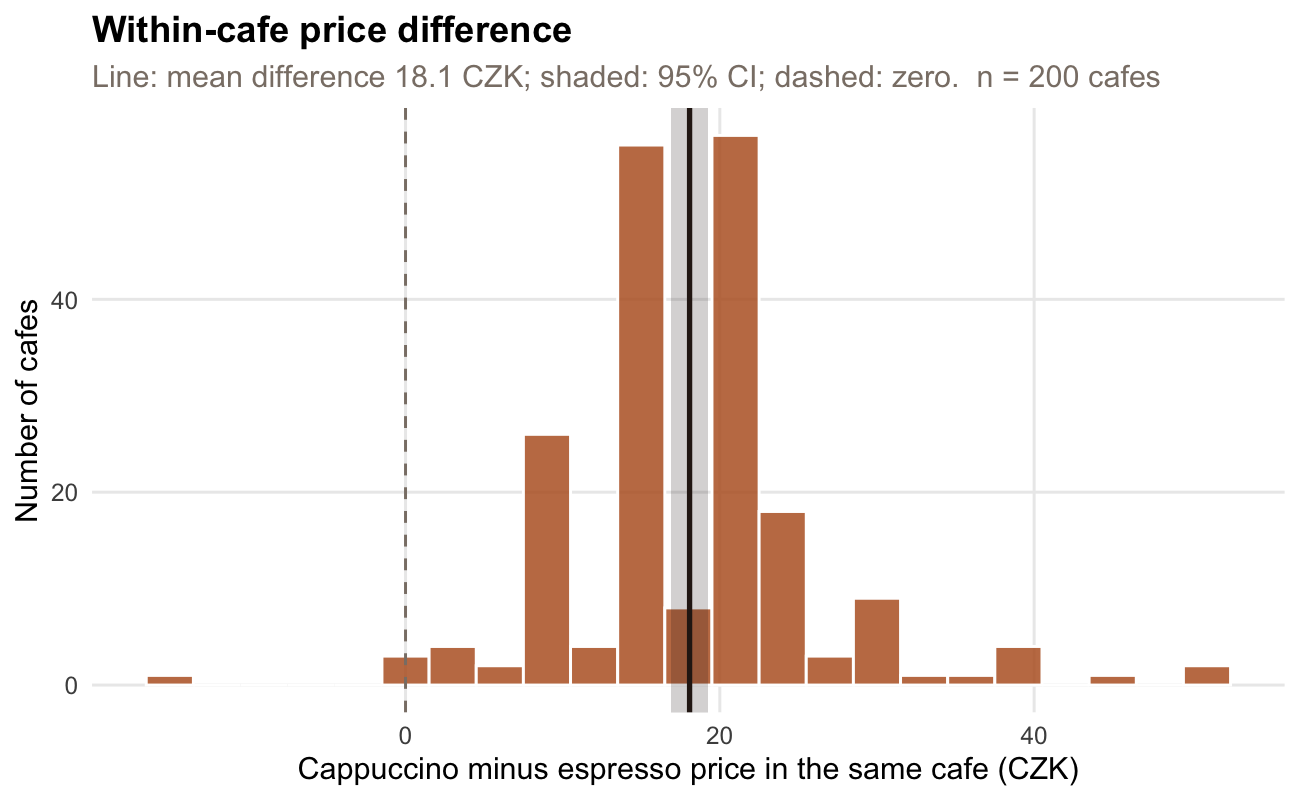
\includegraphics[width=\linewidth]{figures/A3_figure.png}
\column{0.36\textwidth}
\stat{+\AthreeM{} CZK}{cappuccino $-$ espresso, 95\% CI \CI{\AthreeLo}{\AthreeHi}}
\stat{$d_z$ = \AthreeDz}{paired $t$-test, \AthreeP{} (one-tailed)}
\small A1: mean cappuccino \AoneMean{} CZK, 95\% CI \CI{\AoneLo}{\AoneHi}.
\end{columns}
\end{frame}

% 4 ---------------------------------------------------------------
\begin{frame}{Prague 1 is about 6 CZK dearer, but the tests only partly agree}
\begin{columns}[T]
\column{0.6\textwidth}\centering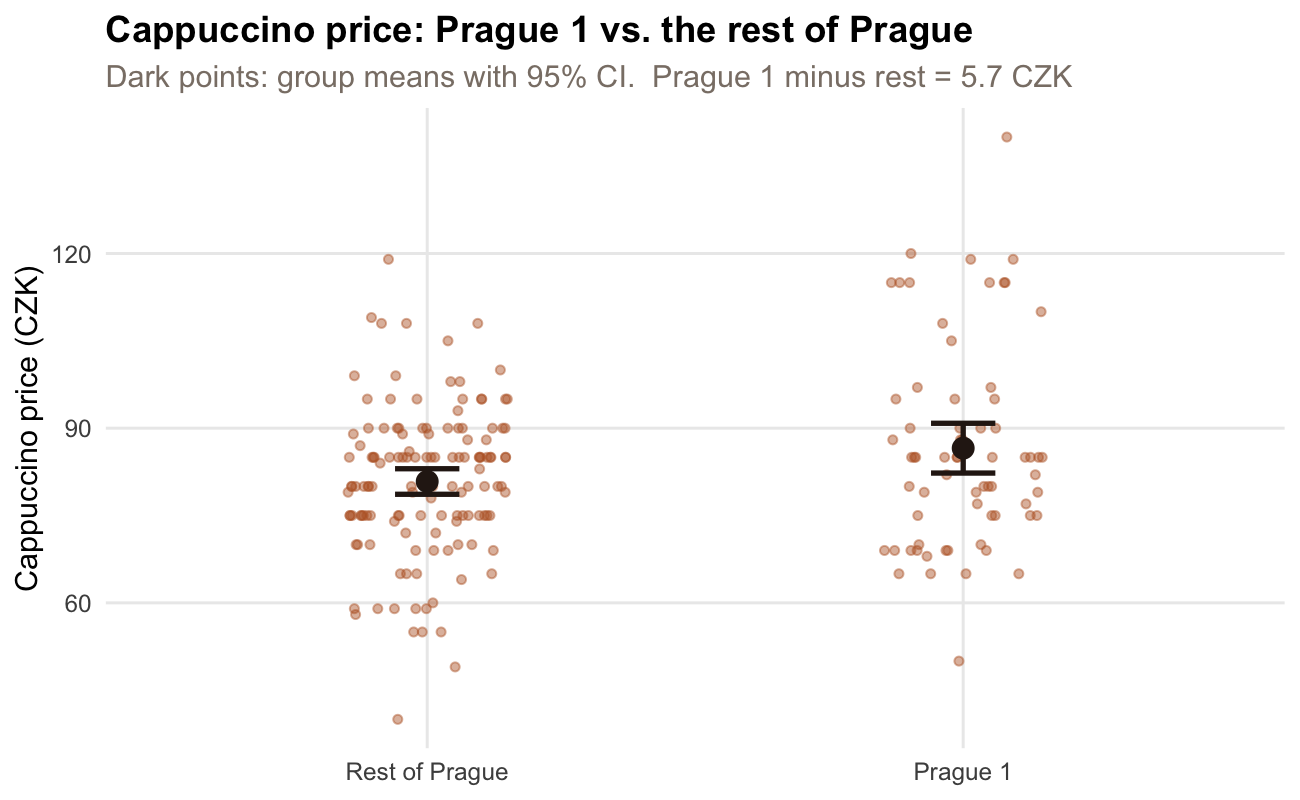
\includegraphics[width=\linewidth]{figures/A2_figure.png}
\column{0.36\textwidth}
\stat{+\AtwoDiff{} CZK}{Prague 1 $-$ rest, 95\% CI \CI{\AtwoLo}{\AtwoHi}}
\stat{$d$ = \AtwoD}{Welch $t$-test, \AtwoP{} (one-tailed)}
\small Rank-sum check: \AtwoWP, shift \AtwoHL{} CZK, not significant.
\end{columns}
\end{frame}

% 5 ---------------------------------------------------------------
\begin{frame}{Districts look alike; international chains cluster in Prague 1}
\centering\figs{A4_figure.png}{A5_figure.png}
\begin{itemize}\small\setlength\itemsep{0.3em}
\item Six districts: Welch $F(\AfourDfa,\,\AfourDfb)$ = \AfourF, \AfourP, $\eta^2$ = \AfourEta; no pair differs after adjustment.
\item Caf\'e type vs Prague 1: Fisher \AfiveFisherP, $V$ = \AfiveV; \AfiveKInt{} of \AfiveNInt{} international chains are in Prague 1.
\end{itemize}
\end{frame}

% 6 ---------------------------------------------------------------
\begin{frame}{Price falls with distance, but only weakly}
\begin{columns}[T]
\column{0.6\textwidth}\centering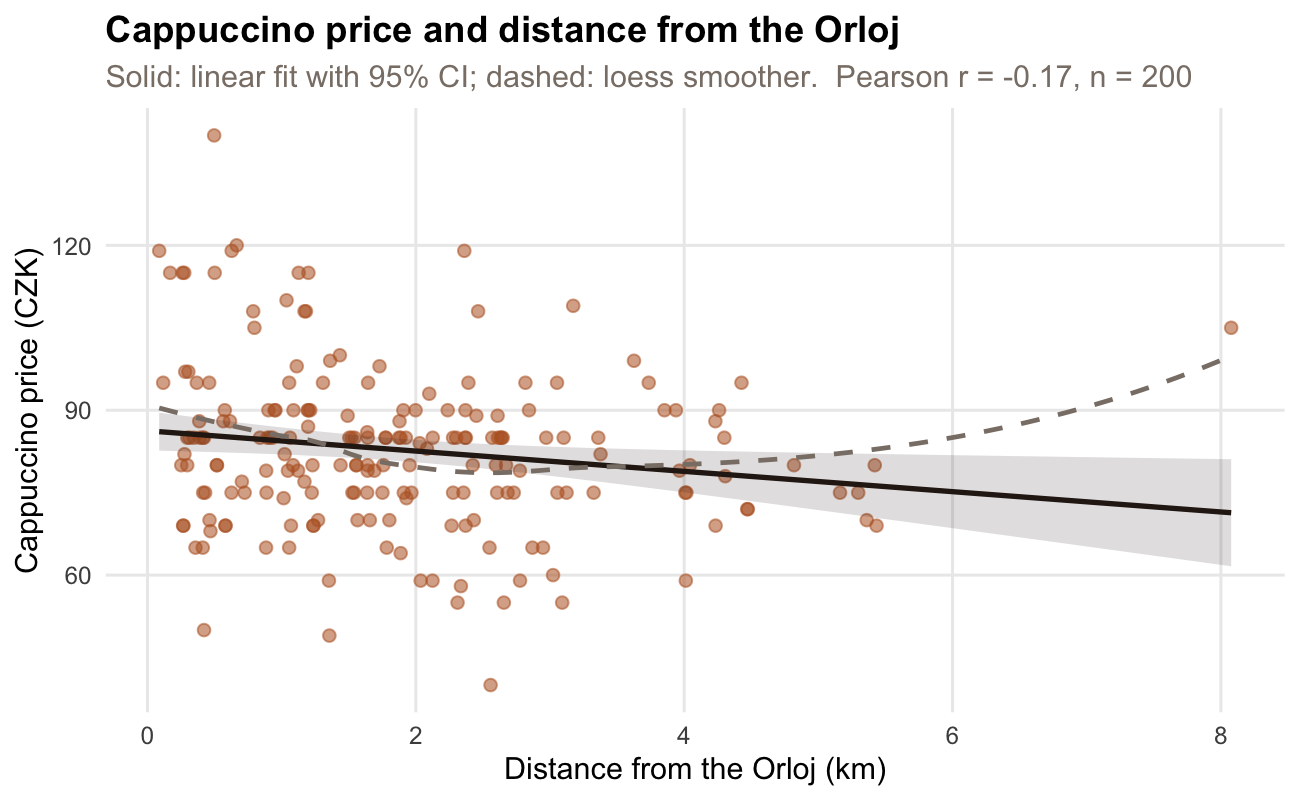
\includegraphics[width=\linewidth]{figures/A6_figure.png}
\column{0.36\textwidth}
\stat{$r$ = \AsixR}{Pearson, 95\% CI \CI{\AsixRLo}{\AsixRHi}}
\stat{\AsixP}{one-tailed; distance shares \AsixRsq\% of price variance}
\small Spearman $\rho$ = \AsixRho{} and Kendall $\tau$ = \AsixTau{} agree.
\end{columns}
\end{frame}

% 7 ---------------------------------------------------------------
\begin{frame}{About 2 CZK per km, and it survives controlling for caf\'e type}
\centering\figs{A7_figure.png}{A8_figure.png}
\begin{itemize}\small\setlength\itemsep{0.3em}
\item A7: \AsevenPct\% per km (robust CI \CI{\AsevenPctLo}{\AsevenPctHi}, \AsevenLogP); \AsevenB{} CZK per km.
\item A8: slope barely moves with caf\'e type; type adds $\Delta R^2$ = \AeightDeltaR{} (\AeightP); local chains +\AeightLocal{} CZK.
\end{itemize}
\end{frame}

% 8 ---------------------------------------------------------------
\begin{frame}{Slopes don't clearly differ by type; farther caf\'es are less likely to be dear}
\centering\figs{A9_figure.png}{A10_figure.png}
\begin{itemize}\small\setlength\itemsep{0.3em}
\item A9: interaction \AnineInt{} CZK/km, CI \CI{\AnineIntLo}{\AnineIntHi}, \AnineP; no clear difference.
\item A10: \AtenAME{} percentage points per km (CI \CI{\AtenAMELo}{\AtenAMEHi}, \AtenP); OR \AtenOR.
\end{itemize}
\end{frame}

% 9 ---------------------------------------------------------------
\begin{frame}{Take-aways}
\renewcommand{\arraystretch}{1.9}
\begin{tabular}{@{}p{2.2cm}p{10cm}@{}}
\colorbox{copper}{\color{white}\bfseries\ Baseline\ } & Cappuccino $\approx$ \AoneMean{} CZK; +28\% over espresso (A1, A3)\\
\colorbox{copper}{\color{white}\bfseries\ Centre\ } & Prague 1 $\approx$ +6 CZK; tests partly disagree (A2)\\
\colorbox{copper}{\color{white}\bfseries\ Distance\ } & $-$2 CZK or $-$2\% per km; weak, CI touches 0 (A6--A8, A10)\\
\colorbox{copper}{\color{white}\bfseries\ Type\ } & Chains charge more; slope the same for both (A8, A9)\\
\colorbox{copper}{\color{white}\bfseries\ Districts\ } & No clear differences (A4)\\
\end{tabular}
\end{frame}

% 10 --------------------------------------------------------------
{\setbeamercolor{background canvas}{bg=espresso}\setbeamercolor{normal text}{fg=white}\setbeamercolor{itemize body}{fg=white}
\begin{frame}[plain]
\color{white}
\vspace{1.2cm}
{\Huge\bfseries What the data cannot tell us\par}
\vspace{0.8cm}
\begin{itemize}\Large\setlength\itemsep{0.7em}
\item \color{white}Convenience sample from ten students, not random caf\'es.
\item \color{white}Observational: distance is associated with price, not the cause.
\item \color{white}Caf\'es in a district, and rows by one student, are not independent; standard errors may be too small.
\item \color{white}\Ntests{} tests in total: one borderline $p$-value is not a finding.
\end{itemize}
\end{frame}}

\end{document}
